\section{The in-the-middle algorithm}
This section will present the in-the-middle algorithm for max-sum problems, and the framework of \emph{variable components}, \emph{constraint components} and \emph{constraint updates} employed by the algorithm.
It will provide theoretical results on the feasibility and optimality guarantees provided by the algorithm, and will present two variations of the update procedure used in the algorithm.
Previous improvements to the \gls{lp} formulation will also be applied to the max-sum version.
First, however, the original \gls{lp} algorithm will be reviewed.

\subsection{Original LP formulation}
To provide context for the max-sum formulation of the in-the-middle algorithm and heuristic, the original algorithm as applied to \gls{lp} problems will be briefly described, and explicit pseudo-code for the algorithm will be presented.
Full descriptions of the \gls{lp} variant of the in-the-middle algorithm are available from \textcites{Wedelin95}{Bastert10}.

The algorithm solves an \gls{ilp} problem
\begin{equation}\label{eq:ilp}
	\begin{aligned}
		{}           & \min*{c^\top x} \\
		\text{s.t. } & Ax = b, \\
		{}           & x \in \{0,1\}^n,
	\end{aligned}
\end{equation}
where \(A \in \{0,1\}^{m\times n}\) and \(b\in\N^m\) (a generalization to the case \(A \in \{-1,0,1\}^{m\times n}\) exists).
The idea is to exploit the Lagrangian relaxation of the problem,
\begin{equation}\label{eq:ilp-lagrange}
	\begin{aligned}
		{}           & \min*{c^\top x - y^\top (Ax - b)}\\
		\text{s.t. } & x \in \{0,1\}^n,
	\end{aligned}
\end{equation}
where \(y\) are the Lagrangian multipliers --- once a value of \(y\) has been fixed to \(\hat{y}\) it is easy to find the minimum of this relaxation.
Assuming all reduced costs \(\bar{c} = (c^\top - \hat{y}^\top A)\) are non-zero one may then express an optimal solution \(\hat{x}\) to the original problem, with \(\hat{x}_i = 1\) for \(\bar{c}_i < 0\) and \(\hat{x}_i = 0\) for \(\bar{c}_i > 0\).

The goal of the algorithm is to manipulate \(y\) to minimize \eqref{eq:ilp-lagrange} while maintaining feasibility for \eqref{eq:ilp}.
The basic idea is to, for every single constraint \(j\) of the problem, find the elements in \(\bar{c}\) that correspond to the variables of that constraint (denoted by \(\bar{c}^j\)) and subtract the average of two \emph{critical values} \(r^+\) and \(r^-\).
The critical values are chosen so that at most \(b_j\) of the values in \(\bar{c}^j\) are strictly positive.
If no sign changes occur after visiting each constraint once, the algorithm has converged and a feasible (assuming \(\bar{c} \neq 0\)) and optimal solution has been found.
\Cref{alg:itm-lp} provides complete pseudo-code for this algorithm, and \textcites{Wedelin95}{Wedelin13} provides further theoretical results.

\begin{algorithm}[p]
	\KwIn{\(A \in \{-1,0,1\}^{m\times n}\), \(b\in\N^m\), \(c\in\R^n\)}
	\KwOut{Optimal solution \(\hat{x}\in\{0,1\}^n\) to \cref{eq:ilp} \KwOr{} \(\emptyset\)}
	\(\bar{c} \leftarrow c\) \;
	\(s^j \leftarrow 0\) \;
	\Repeat{no sign changes in \(\bar{c}\)}{
		\For{\(j=1,\dotsc,m\)}{
			\(r \leftarrow \bar{c}^j + s^j\)\;
			\(d \leftarrow r \cdot a_{\cdot,j}^{-1}\)\;
			\(r^+ \leftarrow b_j\text{th largest element of }d\)\;
			\(r^- \leftarrow (b_j+1)\text{th largest element of }d\)\;
			\(\Delta y \leftarrow (r^+_j + r^-_j)/2\) \;
			\(s^j \leftarrow \Delta y \cdot a_{\cdot,j}\) \;
			\(\) \label{alg:itm-lp:deltay} \tct*[r]{Intentionally left blank}
			\(\bar{c} \leftarrow r - s^j\) \;
		}
	}
	\eIf{\(\bar{c} \neq 0\)}{%
		\For{\(i=1,\dotsc,n\)}{
			\leIf{\(\bar{c}_i \leq 0\)}{\(\hat{x}_i\leftarrow1\)}{\(\hat{x}_i\leftarrow0\)}%
		}%
	}{%
		\KwRet{\(\emptyset\)}%
	}

	\caption{
		The in-the-middle algorithm without its heuristic.
		Counting the sign changes may be done efficiently in the final assignment to \(\bar{c}\).
	}
	\label{alg:itm-lp}
\end{algorithm}

The attentive reader will note that the method described by \cref{alg:itm-lp} may produce situations in which \(\bar{c}_i = 0\) for some \(i\), terminating without an integer solution to the original problem.
To address this issue, the algorithm is transformed from being exact to being approximate by introducing a heuristic.
The purpose of the heuristic is to \enquote{nudge} the reduced costs and move them away from \(0\), while still distorting them as little as possible.
This will force an integer solution through what may be interpreted as coordinate search.
A parameter \(\kappa\) is introduced to govern the heuristic: for \(\kappa=0\) there is no approximation and for \(\kappa=1\) there is maximal approximation.

The idea of the heuristic is then to add a small positive value to positive elements \(\bar{c}_i\), and a small negative value to negative ones.
To this end, the empty \cref{alg:itm-lp:deltay} of \cref{alg:itm-lp} is replaced, introducing an assignment
\begin{equation*}
	s^j_i \leftarrow s^j_i \pm \left(\frac{\kappa}{1-\kappa}(r^+_j - r^-_j) + \delta\right)
\end{equation*}
where addition is used when \(r_i - s^j_i \geq 0\) and subtraction otherwise.
This assignment is (as implied) applied to all elements of \(s^j\).
The (small) parameter \(\delta>0\) ensures that elements of \(\bar{c}\) are kept non-zero at all times.

Note that \textcite[\pno~97]{Bastert10} provide a different but equivalent formulation of \cref{alg:itm-lp} with the approximate heuristic.

\subsection{Max-sum formulation}
Working from the \gls{lp} formulation of the in-the-middle algorithm, \textcite{Wedelin08} introduce a similar algorithm for max-sum problems (which they call \emph{cost propagation}).
The formulation is examined further by \textcite[\pno~11\psqq]{Wedelin13}.
This section will describe the max-sum formulation of the in-the-middle algorithm, reference some theoretical results, and provide explicit pseudo-code for the algorithm.

The algorithm considers a max-sum problem
\begin{equation}\label{eq:maxsum}
	\max*[x] \sum_{g_k\in C} g_k(x^k),
\end{equation}
in accordance with \cref{def:max-sum}.
Recalling the \emph{component model} (\cpageref{pg:component-model}), the functions \(g_k\) may be divided into \emph{variable} and \emph{constraint} components --- for instance, the problem
\begin{equation*}
	\max*[x] g_1(x_1) + g_2(x_2) + g_3(x_3) + g_4(x_1, x_2) + g_5(x_2, x_3)
\end{equation*}
has variable components \(g_1, g_2, g_3\) and constraint components \(g_4, g_5\).
While it is possible to implement the algorithm so that all functions \(g_k\) are translated into constraint components, this division has computational advantages in that the variable components may be represented implicitly in a cost variable.
Therefore, to keep the variable and constraint components apart, the former will be denoted by \(\vcomp_1,\dotsc,\vcomp_n\) and the latter by \(\ccomp_1,\dotsc,\ccomp_m\).
The components are then \(\vcomp_i : D_i \mapsto \Rminus \cup \{-\infty\}\) and \(\ccomp_k : D^k \mapsto \Rminus \cup \{-\infty\}\), where each \(\ccomp_k\) is associated with a subset of all variable components as well, as shown by \cref{fig:maxsum-components} (this subset will be called \(\vcomp^j\)).

\begin{figure}[p]
	\centering
	\begin{tikzpicture}[node distance=.25cm and .25cm]
	\begin{scope}[local bounding box=components]
		% Constraint table
		\node (table) {
			\begin{tikzpicture}[scale=.8]
				\draw[step=1,black,thin] (0,0) grid (3,3);
				\node[anchor=center] at ( .5, .5) {\(0\)};
				\node[anchor=center] at ( .5,1.5) {\(0\)};
				\node[anchor=center] at ( .5,2.5) {\(-\infty\)};
				\node[anchor=center] at (1.5, .5) {\(0\)};
				\node[anchor=center] at (1.5,1.5) {\(-\infty\)};
				\node[anchor=center] at (1.5,2.5) {\(0\)};
				\node[anchor=center] at (2.5, .5) {\(-\infty\)};
				\node[anchor=center] at (2.5,1.5) {\(0\)};
				\node[anchor=center] at (2.5,2.5) {\(0\)};
			\end{tikzpicture}
		};
		% Upper variable
		\node[above=of table] (upper-var) {
			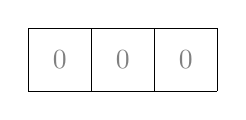
\begin{tikzpicture}[scale=.8]
				\draw[step=1,black,thin] (0,0) grid (3,1);
				\node[anchor=center] at ( .5,.5)
					{\textcolor{gray}{\(0\)}};
				\node[anchor=center] at (1.5,.5)
					{\textcolor{gray}{\(0\)}};
				\node[anchor=center] at (2.5,.5)
					{\textcolor{gray}{\(0\)}};
			\end{tikzpicture}
		};
		% Left variable
		\node[left=of table] (left-var) {
			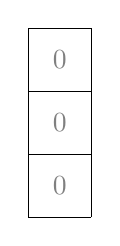
\begin{tikzpicture}[scale=.8]
				\draw[step=1,black,thin] (0,0) grid (1,3);
				\node[anchor=center] at (.5, .5)
					{\textcolor{gray}{\(0\)}};
				\node[anchor=center] at (.5,1.5)
					{\textcolor{gray}{\(0\)}};
				\node[anchor=center] at (.5,2.5)
					{\textcolor{gray}{\(0\)}};
			\end{tikzpicture}
		};
	\end{scope}
	% explanatory texts
	\node[below=of components] (cc-text) {\emph{constraint component \(\ccomp_k(x_i, x_j)\)}}
		(cc-text.east) edge[pointer,bend right=67.5] (table.east);
	\node[above=of components] (vc-text) {\emph{variable components \(\vcomp_i(x_i), \vcomp_j(x_j)\)}}
		(vc-text.east) edge[pointer,bend left=67.5] (upper-var.east)
		(vc-text.west) edge[pointer,bend right=67.5] (left-var.north west);
		%\node[anchor=west] (0, .25) {\emph{constraint component}};
		%\node (2.25, 1) {}
		%	edge[pointer,bend right=22.5] (2.25,1.25) {};
		%
\end{tikzpicture}

	\caption{A single constraint of two variables \(x_i,x_j\) with \(\abs{D}=3\), and consequently a cost table \(g_k(x_i,x_j)\) with nine values. This particular constraint is a hard \emph{all-different} constraint \(x_i\neq x_j\).}
	\label{fig:maxsum-components}
\end{figure}

\begin{algorithm}[p]
	\SetKwFunction{UpdateConstraint}{UpdateConstraint}
	\KwIn{Variable components \(\vcomp_1,\dotsc,\vcomp_n\), constraint components \(\ccomp_1,\dotsc,\ccomp_m\)}
	\KwOut{Feasible solution \(\hat{x}\in X\) to \cref{eq:maxsum} \KwOr{} \(\emptyset\)}
	\lFor{\(i=1,\dotsc,n\)}{\(\bar{\vcomp}_i \leftarrow \vcomp_i\)}
	\lFor{\(j=1,\dotsc,m\)}{\(s^j_i \leftarrow 0\)}
	\Repeat{\(\argmax*[x_i]{\bar{\vcomp}_i(x_i)}\) did not change for any \(i\)}{
		\For{\(j=1,\dotsc,m\)}{
			\(\bar{\vcomp^j}, s^j \leftarrow \text{\UpdateConstraint{\(\ccomp_j\), \(\bar{\vcomp}^j\), \(s^j\)}}\)
		}
	}
	\eIf{\(\argmax*[x_i]{\bar{\vcomp}_i(x_i)}\) is unique for all \(i\)}{%
		\lForEach{\(i=1,\dotsc,n\)}{\(\hat{x}_i \leftarrow \argmax*[x_i]{\bar{\vcomp}_i(x_i)}\)}
	}{%
		\KwRet{\(\emptyset\)}%
	}

	\caption{
		The basic framework of the max-sum in-the-middle algorithm.
		If the constraint updates are non-conflicting, the output is an optimal solution to \cref{eq:maxsum}.
	}
	\label{alg:itm-maxsum}
\end{algorithm}

With this in mind, the basic framework of the algorithm may be introduced (\cref{alg:itm-maxsum}), which intentionally is very similar to that of the \gls{lp} formulation.
Note especially the \emph{modified} variable components \(\hat{\vcomp}_i\), which roughly correspond to the reduced costs \(\bar{c}\) of the \gls{lp} formulation (in the same way that the actual variable components \(\vcomp_i\) roughly correspond to the actual cost vector \(c\)).
% [fix] - Wedelin: "which terminology"

The constraint updates used in the algorithm will now be described and theoretically related to the updates used in the \gls{lp} formulation. In addition to this, some important theoretical results will be mentioned.
Finally, two specific updates will be described.

The basic idea of the constraint update, as with the \gls{lp} formulation, is to modify the variable components in an invariant manner to uniquely identify the (optimal) solution given the constraint component.
This is done by considering only the subproblem consisting of the constraint component \(\ccomp_j\) along with its associated variable components \(\vcomp^j\) and performing a local optimization.
While \textcite[\pno~100\psq]{Wedelin08} present a framework for updates defining a few sought-after properties, only what they call \emph{consistent} and \emph{locally optimal} updates are considered here.
% [fix] - Wedelin: "best terminology?"
These guarantee that any solution found by \cref{alg:itm-maxsum} will be feasible.
Some updates (in particular the fractional \acrshort{dp} update described later, for some parameter values) are additionally \emph{non-conflicting}, which guarantees that any feasible solution found is also optimal.

Each update, as illustrated by \cref{fig:itm-update}, first \emph{moves in} the costs of the variable components into the constraint component (\cref{fig:itm-update:in}, \emph{i.e.} a temporary constraint component \(h_k(x^k) = \ccomp_k(x^k) + \sum_{\vcomp_j \in \vcomp^k} \vcomp_j(x_j)\) is constructed).
Then, costs from the temporary constraint component \(h_k\) are moved out again (\cref{fig:itm-update:out}).
It is mainly this last step that varies between different updates --- it is desirable to move out as much as possible (this improves the convergence rate of the algorithm), but if one moves out too much the \emph{non-conflicting} property is lost and optimality is no longer guaranteed \parencites[\pno~105]{Wedelin08}[\pno~15]{Wedelin13}.

\begin{figure}[t]
	\centering
	\subfloat[Initial constraint\label{fig:itm-update:start}]{\begin{tikzpicture}[node distance=.1cm and .1cm]
	\begin{scope}[local bounding box=components]
		% Constraint table
		\node (table) {
			\begin{tikzpicture}[scale=.6]
				\draw[step=1,black,thin] (0,0) grid (3,3);
				\node[anchor=center] at ( .5, .5) {\footnotesize\(-6\)};
				\node[anchor=center] at ( .5,1.5) {\footnotesize\(0\)};
				\node[anchor=center] at ( .5,2.5) {\footnotesize\(-\infty\)};
				\node[anchor=center] at (1.5, .5) {\footnotesize\(-2\)};
				\node[anchor=center] at (1.5,1.5) {\footnotesize\(-\infty\)};
				\node[anchor=center] at (1.5,2.5) {\footnotesize\(-1\)};
				\node[anchor=center] at (2.5, .5) {\footnotesize\(-\infty\)};
				\node[anchor=center] at (2.5,1.5) {\footnotesize\(-4\)};
				\node[anchor=center] at (2.5,2.5) {\footnotesize\(-1\)};
			\end{tikzpicture}
		};
		% Upper variable
		\node[above=of table] (upper-var) {
			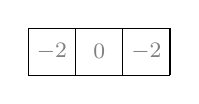
\begin{tikzpicture}[scale=.6]
				\draw[step=1,black,thin] (0,0) grid (3,1);
				\node[anchor=center] at ( .5,.5)
					{\textcolor{gray}{\footnotesize\(-2\)}};
				\node[anchor=center] at (1.5,.5)
					{\textcolor{gray}{\footnotesize\(0\)}};
				\node[anchor=center] at (2.5,.5)
					{\textcolor{gray}{\footnotesize\(-2\)}};
			\end{tikzpicture}
		};
		% Left variable
		\node[left=of table] (left-var) {
			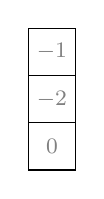
\begin{tikzpicture}[scale=.6]
				\draw[step=1,black,thin] (0,0) grid (1,3);
				\node[anchor=center] at (.5, .5)
					{\textcolor{gray}{\footnotesize\(0\)}};
				\node[anchor=center] at (.5,1.5)
					{\textcolor{gray}{\footnotesize\(-2\)}};
				\node[anchor=center] at (.5,2.5)
					{\textcolor{gray}{\footnotesize\(-1\)}};
			\end{tikzpicture}
		};
		% Move out, left
		\node[below=of table] (dummy) {
			\begin{tikzpicture}[scale=.6,every node/.style={rectangle,rounded corners,fill=white,inner sep=2pt}]
				\node[anchor=center] at (.5, .5)
					{{\scriptsize\textcolor{white}{\(\alpha\)}}};
			\end{tikzpicture}
		};
	\end{scope}
\end{tikzpicture}
}
	\hfil
	\subfloat[The \enquote{move in} operation\label{fig:itm-update:in}]{\begin{tikzpicture}[node distance=.1cm and .1cm]
	\begin{scope}[local bounding box=components]
		% Constraint table
		\node (table) {
			\begin{tikzpicture}[scale=.6]
				\draw[step=1,black,thin] (0,0) grid (3,3);
				\node[anchor=center] at ( .5, .5) {\footnotesize\(-8\)};
				\node[anchor=center] at ( .5,1.5) {\footnotesize\(-4\)};
				\node[anchor=center] at ( .5,2.5) {\footnotesize\(-\infty\)};
				\node[anchor=center] at (1.5, .5) {\footnotesize\(-4\)};
				\node[anchor=center] at (1.5,1.5) {\footnotesize\(-\infty\)};
				\node[anchor=center] at (1.5,2.5) {\footnotesize\(-2\)};
				\node[anchor=center] at (2.5, .5) {\footnotesize\(-\infty\)};
				\node[anchor=center] at (2.5,1.5) {\footnotesize\(-8\)};
				\node[anchor=center] at (2.5,2.5) {\footnotesize\(-4\)};
			\end{tikzpicture}
		};
		% Upper variable
		\node[above=of table] (upper-var) {
			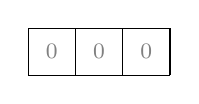
\begin{tikzpicture}[scale=.6]
				\draw[step=1,black,thin] (0,0) grid (3,1);
				\node[anchor=center] at ( .5,.5)
					{\textcolor{gray}{\footnotesize\(0\)}};
				\node[anchor=center] at (1.5,.5)
					{\textcolor{gray}{\footnotesize\(0\)}};
				\node[anchor=center] at (2.5,.5)
					{\textcolor{gray}{\footnotesize\(0\)}};
			\end{tikzpicture}
		};
		% Left variable
		\node[left=of table] (left-var) {
			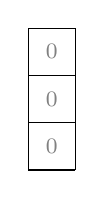
\begin{tikzpicture}[scale=.6]
				\draw[step=1,black,thin] (0,0) grid (1,3);
				\node[anchor=center] at (.5, .5)
					{\textcolor{gray}{\footnotesize\(0\)}};
				\node[anchor=center] at (.5,1.5)
					{\textcolor{gray}{\footnotesize\(0\)}};
				\node[anchor=center] at (.5,2.5)
					{\textcolor{gray}{\footnotesize\(0\)}};
			\end{tikzpicture}
		};
		% Move out, upper
		\node[below=of table] (upper-move) {
			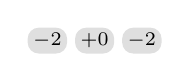
\begin{tikzpicture}[scale=.6,every node/.style={rectangle,rounded corners,fill=gray!25,inner sep=2pt}]
				\node[anchor=center] at ( .5,.5)
					{{\scriptsize\(-2\)}};
				\node[anchor=center] at (1.5,.5)
					{{\scriptsize\(+0\)}};
				\node[anchor=center] at (2.5,.5)
					{{\scriptsize\(-2\)}};
			\end{tikzpicture}
		};
		% Move out, left
		\node[right=of table] (left-move) {
			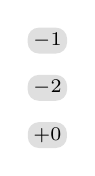
\begin{tikzpicture}[scale=.6,every node/.style={rectangle,rounded corners,fill=gray!25,inner sep=2pt}]
				\node[anchor=center] at (.5, .5)
					{{\scriptsize\(+0\)}};
				\node[anchor=center] at (.5,1.5)
					{{\scriptsize\(-2\)}};
				\node[anchor=center] at (.5,2.5)
					{{\scriptsize\(-1\)}};
			\end{tikzpicture}
		};
	\end{scope}
\end{tikzpicture}
}
	\hfil
	\subfloat[The \enquote{move out} operation\label{fig:itm-update:out}]{\begin{tikzpicture}[node distance=.1cm and .1cm]
	\begin{scope}[local bounding box=components]
		% Constraint table
		\node (table) {
			\begin{tikzpicture}[scale=.6]
				\draw[step=1,black,thin] (0,0) grid (3,3);
				\node[anchor=center] at ( .5, .5) {\footnotesize\(0\)};
				\node[anchor=center] at ( .5,1.5) {\footnotesize\(4\)};
				\node[anchor=center] at ( .5,2.5) {\footnotesize\(-\infty\)};
				\node[anchor=center] at (1.5, .5) {\footnotesize\(2\)};
				\node[anchor=center] at (1.5,1.5) {\footnotesize\(-\infty\)};
				\node[anchor=center] at (1.5,2.5) {\footnotesize\(2\)};
				\node[anchor=center] at (2.5, .5) {\footnotesize\(-\infty\)};
				\node[anchor=center] at (2.5,1.5) {\footnotesize\(0\)};
				\node[anchor=center] at (2.5,2.5) {\footnotesize\(2\)};
			\end{tikzpicture}
		};
		% Upper variable
		\node[above=of table] (upper-var) {
			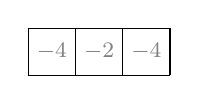
\begin{tikzpicture}[scale=.6]
				\draw[step=1,black,thin] (0,0) grid (3,1);
				\node[anchor=center] at ( .5,.5)
					{\textcolor{gray}{\footnotesize\(-4\)}};
				\node[anchor=center] at (1.5,.5)
					{\textcolor{gray}{\footnotesize\(-2\)}};
				\node[anchor=center] at (2.5,.5)
					{\textcolor{gray}{\footnotesize\(-4\)}};
			\end{tikzpicture}
		};
		% Left variable
		\node[left=of table] (left-var) {
			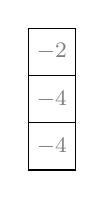
\begin{tikzpicture}[scale=.6]
				\draw[step=1,black,thin] (0,0) grid (1,3);
				\node[anchor=center] at (.5, .5)
					{\textcolor{gray}{\footnotesize\(-4\)}};
				\node[anchor=center] at (.5,1.5)
					{\textcolor{gray}{\footnotesize\(-4\)}};
				\node[anchor=center] at (.5,2.5)
					{\textcolor{gray}{\footnotesize\(-2\)}};
			\end{tikzpicture}
		};
		% Move out, upper
		\node[below=of table] (upper-move) {
			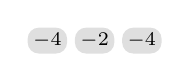
\begin{tikzpicture}[scale=.6,every node/.style={rectangle,rounded corners,fill=gray!25,inner sep=2pt}]
				\node[anchor=center] at ( .5,.5)
					{{\scriptsize\(-4\)}};
				\node[anchor=center] at (1.5,.5)
					{{\scriptsize\(-2\)}};
				\node[anchor=center] at (2.5,.5)
					{{\scriptsize\(-4\)}};
			\end{tikzpicture}
		};
		% Move out, left
		\node[right=of table] (left-move) {
			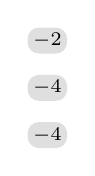
\begin{tikzpicture}[scale=.6,every node/.style={rectangle,rounded corners,fill=gray!25,inner sep=2pt}]
				\node[anchor=center] at (.5, .5)
					{{\scriptsize\(-4\)}};
				\node[anchor=center] at (.5,1.5)
					{{\scriptsize\(-4\)}};
				\node[anchor=center] at (.5,2.5)
					{{\scriptsize\(-2\)}};
			\end{tikzpicture}
		};
	\end{scope}
\end{tikzpicture}
}
	\caption{An illustration of a constraint update (in this case a \gls{dp} update). Note that this particular update is \emph{conflicting}, which results in a lost optimality guarantee.}
	\label{fig:itm-update}
\end{figure}

\subsubsection{The DP constraint update}
\begin{algorithm}[t]
	\SetKwFunction{UpdateConstraint}{UpdateConstraint}
	\Fn{\UpdateConstraint{\(\ccomp_k\), \(\bar{\vcomp}^k\), \(s^k\)}}{
		\KwData{A constraint component \(\ccomp_k\), variable components \(\bar{\vcomp}^k\) and offsets \(s^k\)}
		\KwResult{Updated variable components \(\bar{\vcomp}'^k\) and offsets \(s'^k\)}
		\lForAll{\(\bar{\vcomp}_j\in \bar{\vcomp}^k\)}{\(r^k_j \leftarrow \bar{\vcomp}_j - s^k_j\)}
		\(h_k(x^k) \leftarrow \ccomp_k(x^k) + \sum_{r_j \in r^k} r_j(x_j)\) \;
		\lForAll{\(\bar{\vcomp}_j\in \bar{\vcomp}^k\)}{\(\bar{\vcomp}'_j(x_j) \leftarrow \max*[x\in x^k\setminus x_j]{h(x)}\)}
		\lForAll{\(\bar{\vcomp}'_j\in \bar{\vcomp}'^k\)}{\(s'^k_j \leftarrow \bar{\vcomp}'_j - r^k_j\)}
		\Return{\(\bar{\vcomp}'^k,s'^k\)}
	}
	
	\caption{
		The \gls{dp} constraint update.
	}
	\label{proc:dp-update}
\end{algorithm}
The first update considered is the \gls{dp} update (\cref{proc:dp-update,fig:itm-update}).
It is a fairly unsophisticated update, which extracts the max-marginals along each dimension of the constraint component \(\ccomp_k\) and moves this amount into the corresponding variable component \(\vcomp_i(x_i)\) (\emph{i.e.} the new variable component value becomes \(\bar{\vcomp}'_i(x_i) = \max*[x\in x^k\setminus x_i]{h(x)}\) for every variable component \(\vcomp_i\) and value \(x_i\in D_i\)).
While this should ensure quick convergence since it in effect moves out as much as possible, the update isn't non-conflicting \parencite[\pno~105]{Wedelin08}, which means optimality cannot be guaranteed.

\subsubsection{The fractional DP constraint update}
\begin{algorithm}[t]
	\SetKwFunction{UpdateConstraint}{UpdateConstraint}
	\Fn{\UpdateConstraint{\(\ccomp_k\), \(\bar{\vcomp}^k\), \(s^k\)}}{
		\KwData{A constraint component \(\ccomp_k\), variable components \(\bar{\vcomp}^k\) and offsets \(s^k\)}
		\KwResult{Updated variable components \(\bar{\vcomp}'^k\) and offsets \(s'^k\)}
		\lForAll{\(\bar{\vcomp}_j\in \bar{\vcomp}^k\)}{\(r^k_j \leftarrow \bar{\vcomp}_j - s^k_j\)}
		\(h_k(x^k) \leftarrow \ccomp_k(x^k) + \sum_{r_j \in r^k} r_j(x_j)\) \;
		\lForAll{\(\bar{\vcomp}_j\in \bar{\vcomp}^k\)}{\(\bar{\vcomp}'_j(x_j) \leftarrow \alpha\max*[x\in x^k\setminus x_j]{h(x)}\)} \label{proc:frac-dp-update:diffline}
		\lForAll{\(\bar{\vcomp}'_j\in \bar{\vcomp}'^k\)}{\(s'^k_j \leftarrow \bar{\vcomp}'_j - r^k_j\)}
		\Return{\(\bar{\vcomp}'^k,s'^k\)}
	}
	
	\caption{
		The fractional \gls{dp} constraint update. Note that the only difference between this and \cref{proc:dp-update} is on \cref{proc:frac-dp-update:diffline}.
	}
	\label{proc:frac-dp-update}
\end{algorithm}
Since the regular \gls{dp} update cannot guarantee optimality, it is interesting to see if it may be modified to provide such a guarantee.
\Textcite[\pno~105\psqq]{Wedelin08} provide some theory useful in the construction of non-conflicting updates, in particular a weak upper bound on the amount possible to move out.
They also introduce the \emph{fractional} \gls{dp} update (\cref{proc:frac-dp-update}), which is very similar to the regular \gls{dp} update --- instead of moving out the max-marginals of the constraint component, a fraction \(\alpha\) of the max-marginal is moved out (\emph{i.e.} the new variable component value becomes \(\bar{\vcomp}'_i(x_i) = \alpha\max*[x\in x^k\setminus x_i]{h(x)}\)).

It is immediately obvious that \(\alpha=1\) corresponds to the regular \gls{dp} update, and therefore this will be used as an upper limit of the parameter\footnote{However, note that values \(\alpha>1\) are in no way prohibited by the algorithm and may prove meaningful in some situations.}.
Additionally, \textcite{Wedelin08} provide an upper bound for \(\alpha\) that guarantee non-conflicting updates \parencite[\pno~107]{Wedelin08}.
This upper limit is \(\alpha=\sfrac{1}{n}\), where \(n\) is the number of variables associated with the constraint component (\emph{e.g.} \(n=2\) for the constraint component in \cref{fig:itm-update}).
Interesting values of \(\alpha\) for parameter sweep schemes are thus \(\alpha\in[n^{-1},1]\).

\subsection{Extensions and improvements}
Previous work on the \gls{lp} formulation of the in-the-middle algorithm has yielded useful improvements in performance, and it is therefore interesting to apply these variants to the max-sum variant as well.
Two such improvements are presented.

First, a modification of the \gls{lp} algorithm introduced by \textcite{Bastert10} is considered.
Then, an important addition to the algorithm designed to break ties in variables is introduced.

\subsubsection{The \enquote{push} operation}
In their paper examining the in-the-middle algorithm, \textcite{Bastert10} introduce a \enquote{push} operation intended to improve the quality of any non-optimal solutions found by the approximate algorithm \parencite[\pno~99\psq]{Bastert10}.
The operation is aimed at improving the solution by modifying the reduced costs \(\bar{c}\) to make them \enquote{more similar} to \(c\), contending that the algorithm in fact optimizes with respect to the reduced costs (to which the approximate variant applies non-invariant changes).
This is done by setting \(\bar{c}\leftarrow\bar{c}+\rho c\) (with \(\rho>0\)) and reducing the parameter \(\kappa\) of the approximate \gls{lp} formulation (\cref{alg:itm-lp}) by a set factor when a feasible solution is found (and \(\kappa>0\)).
Additionally, a flag is set that makes the algorithm treat all constraints as violated \parencite[\pno~100]{Bastert10}.

Given the favourable results of \textcite{Bastert10}, it is interesting to benchmark the operation for the max-sum algorithm as well.
Luckily, the \enquote{push} operation is easily translated to apply to the max-sum formulation of the in-the-middle algorithm.
After encountering a feasible solution (and assuming the optimality guarantee does not apply), the modified variable components \(\bar{\vcomp}_i\) are updated as in the \gls{lp} formulation (\emph{i.e.} \(\bar{\vcomp}_i\leftarrow\bar{\vcomp}_i+\rho\vcomp_i\)), and the parameter \(\alpha\) is reduced in a similar way.

\subsubsection{Tie-breaking using noise}
In some problems --- especially those with few hard constraints --- there may be several solutions in a neighbourhood which have the same objective value.
Such situations may result in the modified variables components \(\bar{\vcomp}_j\) being tied for some variables \(j\), which means the algorithm cannot determine a feasible solution (since the corresponding variable value \(\hat{x}_j\) is ambiguous).
To address this issue, a stochastic tie-breaking mechanism is introduced.

The tie-breaking mechanism considers the modified variable components \(\bar{\vcomp}_j\), in which \(\argmax*[x_j]{\bar{\vcomp_j}(x_j)}\) is non-unique if variable \(x_j\) is ambiguous.
Moving through all the variable components \(\bar{\vcomp}_j\), any element whose value \enquote{too close} (determined by a threshold value \(\epsilon\)) to the maximum value \(M = \max*[x_j]{\bar{\vcomp_j}(x_j)}\) is modified by adding uniformly distributed random noise of magnitude \(\zeta\), \emph{i.e.}
\begin{equation*}
	\bar{\vcomp}'_j(x_j) = \bar{\vcomp}_j(x_j) + \begin{cases}
		u \sgn{\bar{\vcomp}_j(x_j) - M} \quad & \text{if \(\abs{\bar{\vcomp}_j(x_j) - M} \leq \epsilon\)} \\
		0 & \text{otherwise}
	\end{cases}, \quad \forall x_j \in D_j,
\end{equation*}
where \(u \in \mathcal{U}(-\zeta,\zeta)\) is a random variable taken from a uniform distribution.
If noise has been added in a previous iteration, that noise is removed from the variable component first.

\subsection{Interpretation in a WCSP context}
The framework commonly employed in \gls{wcsp} optimization focuses on providing equivalence-preserving transformations of the problem graph, in order to obtain good upper and lower bounds which are then used in branch-and-bound strategies.
A fairly thorough presentation of the \emph{arc consistency} notions used in this framework is given by \textcite{Cooper10}.

The notion of \emph{generalized arc consistency} \parencite[\pno~7]{Cooper10} is in fact used by the algorithm, corresponding to the \emph{consistent} updates introduced by \parencite[\pno~101]{Wedelin08}.
This type of arc consistency is normally not utilized in \gls{wcsp} theory, since it is rather weak.
Stronger notions, such as \emph{(full) arc consistency} and \emph{existential arc consistency} \parencite{deGivry05}, are centred around providing very good bound on the problem by projecting costs away from constraints and moving them into the variable components or the nullary constraint, which then immediately provides an easily accessible lower bound on the optimal solution.

Algorithms enforcing full arc consistency are in fact very similar to the \emph{non-conflicting} updates proposed by \textcite{Wedelin08}.
\Textcite[\pno~85\psq]{deGivry05} present an algorithm enforcing this property, and the general structure of this algorithm is very similar to the DP update described above.
First, the costs in one of the variable components are moved into the constraint component.
Then (as in the DP update), the max-marginals are calculated and \enquote{moved out} (\emph{projected}) onto the other variable component.
The result is one variable component with mostly zero-value costs, and one variable component with (if possible) no zero-value costs. 
This fact is then used when enforcing another property, \emph{node consistency} \parencite[\pno~7]{Cooper10}, which in effect moves redundant costs from the variable components to the nullary constraint.

\subsubsection{Stronger constraint component updates}
Although the theory behind the in-the-middle algorithm isn't aimed at providing good upper and lower bounds, instead being concerned with providing an optimality guarantee, there is no reason to discard existing theory in the \gls{wcsp} field.
It appears feasible to implement some of the consistency-enforcing algorithms of \textcite{deGivry05} as constraint component updates, and enforcing node consistency could be done once every few iterations independently of the updates (or in a preprocessing stage).
This could provide lower bounds which could be employed as a secondary optimality guarantee, which could be used to measure the optimality gap in situations where potentially conflicting updates are used.

It may therefore be possible or even desirable to extend notions of stronger arc consistency to the in-the-middle algorithm.
